  \documentclass[a4paper, titlepage]{report}
\usepackage[utf8]{inputenc}
\usepackage[T1]{fontenc}
\usepackage[french]{babel}

\usepackage{graphicx} 


\usepackage{lmodern} % Pour changer le pack de police
\usepackage[vlined, longend]{algorithm2e}
\usepackage{multicol}
\usepackage[a4paper, top=2cm, bottom=2cm, left=2cm, right=2cm]{geometry}


\usepackage{wrapfig}
 


\setlength{\algomargin}{0em}
\SetKwRepeat{Repeat}{Do}{While}
\SetKwIF{If}{ElseIf}{Else}{If}{then}{Else if}{Else}{EndIf}
\SetKwFor{For}{For}{do}{Done}
\SetKwFor{While}{While}{do}{Done}

\providecommand{\SetAlgoLined}{\SetLine}
\providecommand{\DontPrintSemicolon}{\dontprintsemicolon}

\SetKwBlock{Begin}{Begin}{End}

\SetKw{KwFrom}{from }
\SetKw{KwBy}{by }
\DontPrintSemicolon	% do not print the ';' symbol
\newcommand{\TRUE}{\textit{TRUE} }
\newcommand{\FALSE}{\textit{FALSE} }
\newcommand{\AND}{\textit{AND} }
\newcommand{\OR}{\textit{OR} }
\newcommand{\NULL}{\textit{NULL} }

\newcommand{\NewWhile}{\SetKwBlock{While}{while}{}}
\newcommand{\NormalWhile}{\SetKwBlock{While}{while}{Done}}

\setcounter{secnumdepth}{5}
\setcounter{tocdepth}{5}

\newenvironment{lexicon}{\noindent \hspace{1.2em} {\bf \underline{Lexicon}} \\~\\}{ ~\\ }
\newenvironment{algo}{\noindent \hspace{1.2em} {\bf \underline{Algorithm}} \\~\\ \begin{algorithm}[H] \SetAlgoLined }{\end{algorithm}  ~\\}

\usepackage{listings}


\title{LO43 
     Flotte de véhicules autonomes}
\author{Buri Theo florian Lacour} 
\date{Hiver 2013}

\makeatletter
\def\clap#1{\hbox to 0pt{\hss #1\hss}}%
\def\ligne#1{%
\hbox to \hsize{%
\vbox{\centering #1}}}%
\def\haut#1#2#3{%
\hbox to \hsize{%
\rlap{\vtop{\raggedright #1}}%
\hss
\clap{\vtop{\centering #2}}%
\hss
\llap{\vtop{\raggedleft #3}}}}%
\def\bas#1#2#3{%
\hbox to \hsize{%
\rlap{\vbox{\raggedright #1}}%
\hss
\clap{\vbox{\centering #2}}%
\hss
\llap{\vbox{\raggedleft #3}}}}%
\def\maketitle{%
\thispagestyle{empty}\vbox to \vsize{%
\haut{}{\@blurb}{}
\vfill
\vspace{1cm}
\begin{flushleft}
\usefont{OT1}{ptm}{m}{n}
\huge \@title
\end{flushleft}
\par
\hrule height 4pt
\par
\begin{flushright}
\usefont{OT1}{phv}{m}{n}
\Large \@author
\par
\end{flushright}
\vspace{1cm}
\vfill
\vfill
\bas{}{\@location, \@date}{}
}%
\cleardoublepage
}
\def\date#1{\def\@date{#1}}
\def\author#1{\def\@author{#1}}
\def\title#1{\def\@title{#1}}
\def\location#1{\def\@location{#1}}
\def\blurb#1{\def\@blurb{#1}}
\date{Décembre 2014}
\author{}
\title{}
\makeatother
\title{LO43 Flotte de véhicule autonomes}
\author{Buri Theo Florian Lacour}
\location{Belfort}
\blurb{%
Université de technologie de Belfort-Montbéliard
}% 

\usepackage{array}
\usepackage[T1]{fontenc}

\usepackage{color}
\definecolor{pblue}{rgb}{0.13,0.13,1}
\definecolor{pgreen}{rgb}{0,0.5,0}
\definecolor{pred}{rgb}{0.9,0,0}
\definecolor{pgrey}{rgb}{0.46,0.45,0.48}

\usepackage{listings}
\lstset{language=Java,
  showspaces=false,
  showtabs=false,
  breaklines=true,
  showstringspaces=false,
  breakatwhitespace=true,
  commentstyle=\color{pgreen},
  keywordstyle=\color{pblue},
  stringstyle=\color{pred},
}


\begin{document}

\maketitle
\tableofcontents
\newpage
\chapter*{Introduction}
\addcontentsline{toc}{chapter}{Introduction}
\hspace{0.5cm}Dans le cadre de  l'UV LO43 " Bases fondamentales de la programmation orientée objet", il nous a été demandé de réaliser un projet de groupe, afin de mettre en pratique les connaissances acquises lors des cours et TDs du semestre.
\\
Trois sujet nous on été présentés. Nous avons fait le choix de traiter le sujet de la "Flotte de véhicules autonomes", et ceci pour plusieurs raisons :
\begin{itemize}
  \item (A TROUVER)
  \item N'étant que deux, sur un maximum de quatre étudiants par groupe autorisés, les autres sujets ne nous ont pas parus réalisables en temps et en heures et sans bugs majeurs...
  \item (A TROUVER)
\end{itemize}
Nous présenterons tout d'abord le sujet, ses contraintes, et les libertés prises par rapport à celles-ci. Par la suite, nous parlerons des différents diagrammes UML, et les expliquerons. Enfin, nous terminerons par l'implémentation en Java et l'interface graphique.


\setcounter{chapter}{1}
\setcounter{section}{1}
\part{ Présentation du sujet}
\section{Objectif}
 Le programme à réaliser consistait en la modélisation d'une flotte de véhicules évoluant dans une infrastructure de circulation partagée. Pour cela, il a tout d'abord fallu modéliser la partie calculatoire à l'aide du langage UML, puis ensuite l'implémenter en Java et lui donner une interface graphique
\section{Reformulation du sujet}
\subsection{Plateau}
Le plateau donné par le sujet est le suivant :
\vspace{0.5cm}

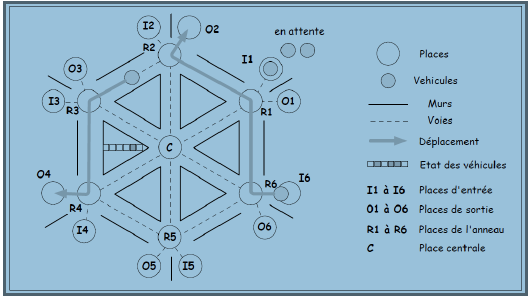
\includegraphics[]{Images/Plateau}
\vspace{0.5cm}
\\
Chaque place, exceptée celle du centre, est rattachée à une place de départ et une place de sortie. Les voitures disposant d'un passager partent depuis une place d'entrée (que celui-ci leur donne) et, à la fin de celle-ci, rejoignent une place de sortie (même chose).\\
La place centrale n'est utilisée que lors d'un trajet reliant deux places opposées...
\subsection{Passagerss et contrôleur}
Chaque passager doit être transporté d'une place à une autre. Pour ce faire, ils envoient une requête au module qui se charge du contrôle du plateau : le contrôleur. Par la suite, celui-ci assignera cette mission à un des véhicules de sa flotte (sous la forme d'un passager, ayant un départ et une arrivée). Celui-ci calculera ensuite le trajet qu'il suivra pour la mener à bien.\\
C'est alors le véhicule qui décide de partir : pour cela il doit envoyer une requête au contrôleur pour savoir si son chemin est déjà réservé. Si ce n'est pas le cas, le contrôleur l'autorise, et le véhicule part. La requête se fait sous la forme d'une Request Map, constituée de booléens indiquant l'intention du véhicule de réserver une place ou non.\\
Pour exemple, lorsqu'une voiture désire aller de la place I1 à O2, elle aura besoin de réserver I1, R1, R2 et O2. La Request Map seras alors la suivante :
\vspace{0.5cm}

\begin{tabular}{|l|l|l|l|l|l|l|l|l|l|l|l|l|l|l|l|l|l|l|l|}

\hline
  I1 & I2 & I3 & I4 & I5 & I6 & R1 & R2 & R3 & R4 & R5 & R6 & O1 & O2 & O3 & O4 & O5 & O6 & C \\
  \hline
   T & F & F & F & F & F & T & T & F & F & F & F & F & T & F & F & F & F & F\\
 \hline

\end{tabular}\\
\vspace{0.25cm}\\
Afin d'éviter toute erreur lors de la réservation, nous avons défini la priorité des places qui suit:
\begin{center}
I1<I2<I3<I4<I5<I6<R1<R2<R3<R4<R5<R6<O1<O2<O3<O4<O5<O6<C
\end{center}
Ceci permettra d'éviter que deux véhicules tentent de réserver la même place à deux moments différents, et que le contrôleur les valide...

\subsection{Contraintes et libertés prises sur le sujet}


S'ajoutent alors quelques contraintes, qui régissent le programme :
\begin{itemize}
  \item Les véhicules ne peuvent utiliser la place centrale qu'à la seule condition qu'ils doivent se rendre à la place en face de la leur.
  \item Une place ou une route (reliant deux places) ne peut être utilisée que par un seul et unique véhicule.
  \item Un véhicule qui souhaite emprunter un chemin occupé doit attendre que celui-ci se libère.
\end{itemize}
\vspace{0.25cm}
Ainsi, par rapport à ces différentes consignes, nous avons choisi de prendre certaines libertés :
\vspace{0.25cm}
\begin{itemize}
  \item Un véhicule ne peut pas contourner une place occupée pour mener sa mission à bien.
  \item 
\end{itemize}
\setcounter{chapter}{0}
\setcounter{section}{0}
\part{Conception UML}
%non de chapitre a changer

\chapter{Les Diagramme UML}
\section{Diagramme des cas d'utilisation (annexe A)}
\hspace{0.5cm} Le diagramme des cas d'utilisation permet de représenter les actions que l'utilisateur peut faire. Dans notre projet, en lançant le programme, l'utilisateur a plusieurs solutions :
\begin{itemize}
\item Voir les crédits (c'est à dire les auteurs du programme, nous)
\item Choisir de jouer en mode manuel, dans ce cas il devras par la suite choisir lui-même les missions attribuées aux véhicules.
\item Jouer en simulation, dans ce mode toutes les requête sont générées par le programme : l'utilisateur se contente de regarde la simulation s'opérer.
\item Avoir accès aux options : une fois dans ce menu, il peut choisir de changer la rapidité des voitures.
\end{itemize}
Nous avons choisi de diviser l'utilisateur principal en deux autres : un utilisateur qui utiliserait le mode manuel, et un autre qui utiliserait le mode automatique. Ceci étant dû au fait que l'utilisateur en mode manuel pourra accéder à des fonctions interdites au mode automatique (la création d'un passager).\\
En outre, une fois sur l'écran de "jeu" (où se déplacent les véhicules), l'utilisateur (et quel que soit son mode) pourra mettre la simulation en pause et, si nécessaire, réinitialiser celle-ci. 
\section{Diagramme de séquence(annexe B)}
\hspace{0.5cm} Le diagramme de séquence permet de représenter les interactions entre les différentes classes selon un ordre chronologique.
\section{Diagramme de classes(annexe C)}
\hspace{0.5cm} Nous verrons en détail, une description de chaque classe.

\chapter{Description des classes}
\section{Classe BoiteAuxLettre}
     
      Il s'agit de la classe recevant toute les requêtes, qu'elles soient envoyées depuis la partie graphique (c'est à dire des requêtes pour la création d'une nouvelle mission, et donc d'un nouveau passager), ou du modèle. Il y a 4 requêtes différentes, stockées chacunes dans une liste différente:
      \begin{wrapfigure}[17]{l}{5.5cm}
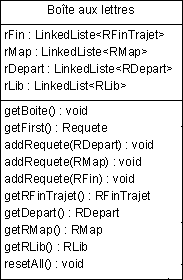
\includegraphics[scale=1]{Images/boite.png}
\end{wrapfigure} \\  
      \begin{itemize}
      \item Une liste de requêtes de départ : cette liste contient toutes les demandes de trajet. Ces trajet peuvent être demandés soit par l'utilisateur, soit générés par le modèle.
      \item Une liste de requêtes de trajet : ce sont les requêtes qu'envoient chacun des véhicules ayant un passager pour demander au contrôleur la permission d'utiliser un chemin (la réponse n'est positive que si le chemin concerné est libre)...
      \item Une liste de requêtes de fin de trajet : ce sont les requête qu'envoient les véhicules lorsqu'ils ont mené leur mission à bien (et donc qu'ils sont arrivés à leur place d'arrivée). Elles permettent alors de libérer le véhicule.
      \item Enfin, une liste de requêtes de libération de ressources : ces requêtes sont envoyées par les véhicules lorsqu'il n'ont plus besoin d'une place (lorsqu'ils sont déjà passés de dessus). Le contrôleur peut alors considérer ces places comme disponibles.
      \end{itemize}


\section{La classes Contrôleur}



Il s'agit de la classe principale : c'est elle qui s'occupe de gérer les déplacements des différents véhicules sur la carte. Le contrôleur a directement accès à la boîte aux lettres, et donc aux requêtes qu'elle contient.\\
C'est également lui qui possède la "carte" (ici, une HashMap) des différentes places du réseau routier : il est le seul à agir dessus.
La méthode traiteRequete() se charge de traiter les requêtes selon leur priorité :
\begin{wrapfigure}[16]{l}{5cm}
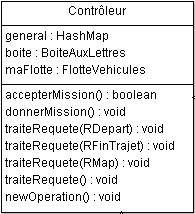
\includegraphics[scale=1]{Images/controleur.png}
\end{wrapfigure}
 \begin{itemize}
      \item Les requêtes de fin de trajet sont prioritaires sur toutes les autres : rendre un véhicule à nouveau disponible signifie le débarquement d'un passager, et donc la capacité d'en accepter de nouveaux.
      \item Les requêtes de libération de ressources arrivent en second. En effet, rendre une place disponible le plus vite possible est prioritaire pour pouvoir valider les trajets d'autres véhicules.
      \item Viennent ensuite les requêtes de départ, permettant aux passagers d'être pris en charge plus vite que les requêtes de trajet, bien plus nombreuses.
      \item Les requêtes de trajet sont les moins prioritaires, notamment en raison de le nombre : en effet, elles sont générées à intervalle régulier par les véhicules, jusqu'à ce qu'ils aient pu emprunter le chemin qu'ils désirent.
      \end{itemize}

Par la suite, et en fonction des requêtes qu'il reçoit, le contrôleur a plusieurs tâches. Il peut libérer un véhicule en fin de trajet, en réserver un autre et lui attribuer un passager. Enfin, il valide (ou non) les chemins demandés par les véhicules, et se charge ensuite de réserver les ressources correspondantes.
\section{Les classes Requêtes}

Etant donné que le but de chaque requête a été explicité ci-dessus, et que la structure de celles-ci ne présente pas d'intérêt particulier, nous nous intéresserons à leurs caractéristiques générales. \\
Chaque type de requêtes a sa propre liste, contenue dans la boîte aux lettres. Un requête, une fois traitée, est immédiatement détruite. Enfin,à chaque liste de requêtes est attribuée une priorité, afin que le contrôleur traite les requêtes les plus importantes en premier.

\section{La classe Cerveau}
\begin{wrapfigure}[10]{l}{4.5cm}
\vspace{-0.5cm}
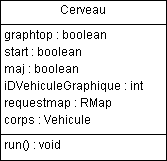
\includegraphics[scale=1]{Images/cerveau.png}
\end{wrapfigure}Il s'agit du Thread chargé de négocier le départ puis l'arrivée d'un véhicule. Il est ajouté au véhicule lorsque celui-ci reçoit un passager. C'est alors lui qui se charge, après avoir calculé le chemin à emprunter, de faire la demande de réservation auprès du contrôleur et, si celui-ci l'autorise, à faire partir le véhicule. Cette autorisation se fait par le biais d'un booléen, modifié par la flotte de véhicules, à la demande du contrôleur.\\
Par la suite, il se charge d'acheminer le véhicule jusqu'à sa destination, et signale ensuite au contrôleur la fin du trajet. Il est alors détruit, et le véhicule devient à nouveau disponible. Celui-ci recevra un nouveau "Cerveau" lors de l'embarquement du passager suivant.
\vspace{0.3cm}
En parallèle, le cerveau se charge également de synchroniser l'avancée du trajet avec la partie graphique : en effet, afin d'éviter des bugs d'affichage, le modèle doit attendre que le véhicule affiché atteigne la place suivante avant d'envoyer les requêtes de libération et, à la fin du trajet, la requête de fin de trajet.
\vspace{0.5cm}
\section{La Classe Véhicule}

%\begin{wrapfigure}[16]{l}{5cm}
%\vspace{-0.5cm}
%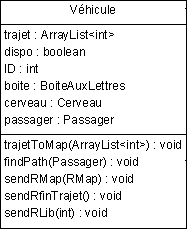
\includegraphics[scale=1]{Images/vehicule.png}
%\end{wrapfigure}
Chaque véhicule possède un identifiant unique donné par la classe "Flotte de Véhicules" et stocké  dans un Integer "identifiant". Les véhicules sont instanciés sans trajet ni cerveau. Ceux-ci lui seront attribués plus tard, la de l'embarquement d'un passager. Le Cerveau se charge alors d'appeler les fonctions du véhicule pour calculer le trajet, envoyer des requêtes...
A la fin de son trajet, seul le cerveau est détruit. Le véhicule  redevient alors libre, dans l'attente d'un nouveau passager.

\part{Implémentation Java}
\chapter{Choix d'architecture}
\section{Le pattern MVC}
Afin de permettre une meilleure représenation des différentes parties du programme, le choix a été fait d'utiliser le pattern "Modèle - Vue - Contrôleur". Il est constitué comme suit :\\
\begin{itemize}
\item La vue est la partie visible pour l'utilisateur : elle rassemble les différentes fenêtres du programme, les boutons et autres moyens pour l'utilisateur d'interagir avec celui-ci.
\item Le contrôleur (afin d'éviter toute confusion avec le nom de la classe principale du programme, nous l'appellerons Vérificateur)se charge de vérifier  que les données venant de la vue (et donc souvent de l'utilisateur), afin d'éviter l'envoi d'arguments non attendus aux fonctions internes. Il se charge par la suite de transmettre ces données au modèle.
\item Le modèle est la partie calculatoire du programme. C'est lui qui, dans notre cas, se charge de la totalité de la simulation (voitures, contrôleur, trajets, etc...). Il peut alors envoyer des données à la vue pour qu'elle les affiche (faire bouger un véhicule, par exemple).
\end{itemize}
Ces trois parties sont mises en relation par le biais d'interfaces "Observer" et "Observable", qui permettent au modèle d'envoyer des informations à la vue sans même avoir conscience de son existence. Cette indépendance permet de modifier la vue à volonté sans avoir à modifier le modèle...
\section{Des threads pour régir les déplacements}

Nous avons fait le choix d'utiliser des Threads pour permettre à chaque véhicule de bouger indépendamment.

\chapter{Difficultés rencontrées}

\chapter{Fonctions importantes}
Ce chapitre est destiné à mettre plus en lumières certaines fonctions que nous avons jugé assez importantes pour nous y attarder. Nous en donnerons le code, puis expliciterons sa fonction et son fonctionnement.
\section{Classe Controleur}
La fonction principale de cette classe et la méthode traiteRequete : en effet il s'agit de la méthode qui doit se charger de vérifier si il y a des requêtes dans la boîte aux lettres et, si c'est le cas, effectuer un traitement différent selon la nature de la requête. De plus, les requêtes n'étant pas toutes envoyées en même temps, il est possible que le contrôleur aie à attendre l'arrivée d'une requête...\\

Nous pouvont alors nous attarder sur la méthode traiteRequete(RMap). Cette méthode doit, dans un premier temps vérifier que toutes les places demandées sont libres, puis elle doit les réserver dans la hashmap génerale. Elle se charge également de signaler à la voiture qu'elle peut (ou non) partir...
\begin{lstlisting}
private void traiteRequete(RMap r) {
	ArrayList<Boolean> m = r.getRequest_map();
	// compteur pour savoir ou on en est dans les boucles
	int i = 0;
	// il y aura au maximum 5 routes de reserver+ l'ietreateur sur ce
	// tableau
	int[] tab = new int[5];
	int iterateurTab = 0;
	// entier pour savoir combien de true il y a dans la requestMapr e
	// general
	int trueInRequete = 0;
	// entie pour connaitre le nombre de true dans la liste general;
	int trueInGeneral = 0;
	for (Boolean b : m) {
		if (b == true) {
			trueInRequete++;
			// si la place est libre
			if (general.get(i)) {
				trueInGeneral++;
				tab[iterateurTab] = i;
				iterateurTab++;
			}
		}
		i++;
	}
	// si le nombre true dans la request map et dans la hasmap general sont
	// egaux alors les ressource sont libre et on peut les reserver+passer le boolean de la voiture en true
	if(trueInRequete==trueInGeneral){
		//fonction permettant de de metre les ressource en indisponibilite
		for(int j=0;j<i;j++){
			general.put(tab[i], false);
		}
		maFlotte.lancerVehicule(r.getIdentifiant(), true);	
	}
}
\end{lstlisting}
\section{Classe Vehicule}
Une des méthodes les plus importantes de cette classe est la méthode findPath qui, à partir d'un passager et des informations qu'il contient, crée une liste de places qui qui constitueront le trajet à suivre par le véhicule. 
Pour cela, il faut tout d'abord faire la différence entre deux cas possibles :\\
\begin{itemize}
\item La place d'arrivée est située en face de la place de départ, auquel cas le trajet passe obligatoirement par le centre.
\item La place d'arrivée est située autre part. En ce cas, il faut alors calculer le chemin le plus rapide pour s'y rendre.
\end{itemize}
\begin{lstlisting}
public void findPath(Passager p) {
	// On vide la liste
	trajet.clear();
	// On stocke les places de depart et de fin (on parle ici des places R,
	// pas des places d'entree ou de sortie)
	int dep = p.getDebut() + 10;
	int fin = p.getFin() + 10;
	int a, b;
	int count = -1;
	// On cree deux tableaux pour parcourir la carte dans les deux sens
	int[] l1 = new int[3];
	int[] l2 = new int[3];
	// On commence par la place de depart (son identifiant est egal a la
	// place R - 10)
	trajet.add(dep - 10);
	// Si la place d'arrivee est en face, on passe par le centre
	if (Math.abs(dep - fin) == 3) {
		trajet.add(dep);
		trajet.add(30);
	} else {
		// On commence a la place R de depart
		a = dep;
		b = dep;
		// Ensuite, on parcoure la carte dans les deux sens pour determiner
		// le chemin le plus rapide
		while (a != fin && b != fin) {
			count++;
			// On stocke le trajet
			l1[count] = a;
			l2[count] = b;
			// On se charge de faire un cycle (le 6 est suivi du 1)
			// S'agissant des places R, leur identifiant est decale de 10
			if (a == 16) {
				a = 10;
			}
			if (b == 11) {
				b = 17;
			}
			// On se decale dans les deux sens
			a++;
			b--;
		}// Si le trajet b est le plus court
		if (b == fin) {
			// On le stocke dans le premier tableau
			l1 = l2;
		}// Enfin, on stocke le trajet dans la liste
		for (int i = 0; i < l1.length; i++) {
			if (l1[i] != 0) {
				trajet.add(l1[i]);
			}
		}
	}
	// On termine par la place R finale, puis la place d'arrivee (R + 10)
	trajet.add(fin);
	trajet.add(fin + 10);
}
\end{lstlisting}
Grace à cette liste de points,  la classe va pouvoir générer une RMap qui seras par la suite envoyée à la boîte aux lettres, formatée comme indiqué  dans la partie Requête.

\chapter*{Conclusion}



\section{Classe Boite au lettres}
Cette classe possede 4 listes, chacune de ces liste a le méme logique: dans un premier temps le controleur doit pouvoir acceder a la taille de cette liste afin de savoir si elle est vide ou non.
\\
De plus  lorsque le controleur veut une requete il faut lui envoyer puis suprimer cette requete de la liste. Voici un exemple d'implementatio pour la methode getDepart

\begin{lstlisting}
public RDepart getDepart() {
	RDepart r = new RDepart();
	// on recupere le sernier element
	r.clone(rDepart.get(rDepart.size() - 1));
	rDepart.remove(getSizeRDepart() - 1);
	return r;
}
\end{lstlisting}

\chapter*{Conclusion}
Grace a ce projet vous avont pus nous faire une modélisation de notre projet a l'aide de l'UML, ceci nous a permit d'engager un travail de reflexion de notre projet en amont, et donc nous economiser du temps sur une eventuel faute d'architecture que l'on aurait pus commetre sans ce langage. De plus grace a ce projet nous avont pus voir de nouvelle fonctionlaiter de JAVA qui sont les Thread et les exception. Enfin nous avont implementer dans ce projet la javadoc afin que la communication entre les différents devellopeur soit plus simple. Nous avont aussi utiliser git pour stocker notre projet, nous avont choisi cette outil car il permet une gestion simple des différente version, ainsi qu la possibilité de travailler en méme temps sur le projet sans conflit.
%  les annexesra
\appendix
%diagrame cas d'utilisation
\chapter*{Annexe A}
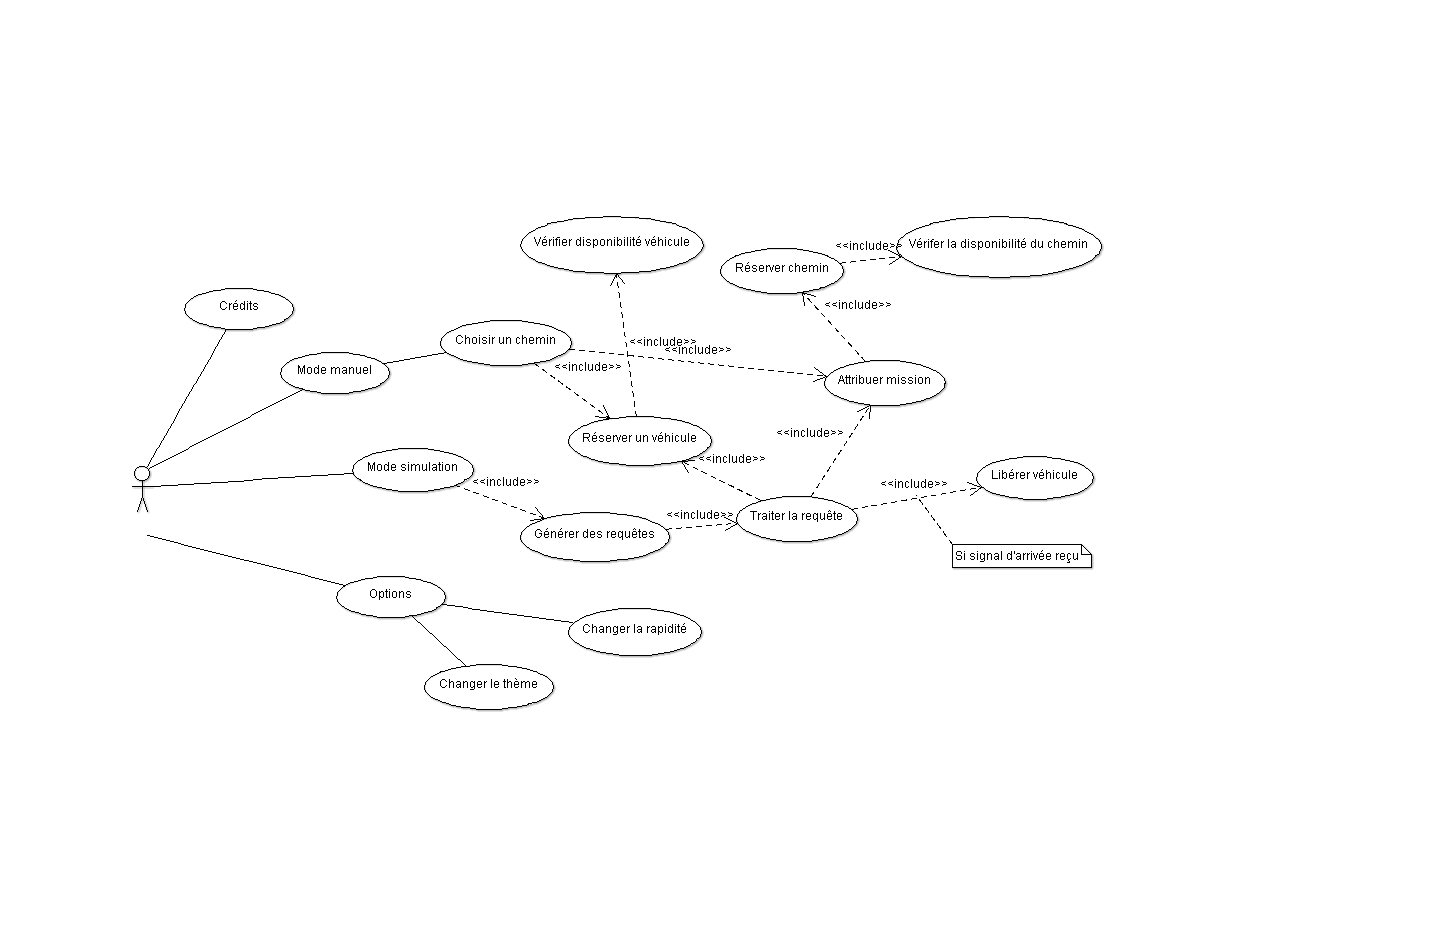
\includegraphics[width=455px, height=190px]{Images/CasUtilisation.PNG}
%diagrame de sequence
\chapter*{Annexe B}
\end{document}